
%(BEGIN_QUESTION)
% Copyright 2015, Tony R. Kuphaldt, released under the Creative Commons Attribution License (v 1.0)
% This means you may do almost anything with this work of mine, so long as you give me proper credit

\noindent
{\bf Lab Exercise -- introduction}

\vskip 5pt

Your task is to build, document, and calibrate a {\it split range} valve system with another team, where a pair of control valves are controlled by the output of a single pneumatic controller in its ``manual'' mode.  Each control valve will use a pneumatic positioner (not an electronic positioner!) to implement the split-ranges.  Each instrument in the loop should be labeled with a proper tag name (e.g. ``HV-78a'' and ``HV-78b'' for two split-ranged, hand-controlled valves), with all instruments in each loop sharing the same loop number.  Write on pieces of masking tape to make simple labels for all the instruments and signal lines.

An additional objective of this lab is to properly cut, bend, and fit metal instrument tubing.  Each student is to bend a length of copper or stainless-steel tubing somewhere in their pneumatic controller/valve system and demonstrate to the instructor that the tubes all fit neatly (right-angle corners, proper offsets, level and plumb).  Instrument tube bending is something of an art, and requires practice to master.

The following table of objectives show what you and your team must complete within the scheduled time for this lab exercise.  Note how some of these objectives are individual, while others are for the team as a whole:

\underbar{Objective completion table:}

% No blank lines allowed between lines of an \halign structure!
% I use comments (%) instead, so that TeX doesn't choke.

$$\vbox{\offinterlineskip
\halign{\strut
\vrule \quad\hfil # \ \hfil & 
\vrule \quad\hfil # \ \hfil & 
\vrule \quad\hfil # \ \hfil & 
\vrule \quad\hfil # \ \hfil & 
\vrule \quad\hfil # \ \hfil & 
\vrule \quad\hfil # \ \hfil & 
\vrule \quad\hfil # \ \hfil \vrule \cr
\noalign{\hrule}
%
% First row
{\bf Performance objective} & {\bf Grading} & {\bf 1} & {\bf 2} & {\bf 3} & {\bf 4} & {\bf Team} \cr
%
\noalign{\hrule}
%
% Another row
Team meeting and prototype sketch (do {\it first!}) & mastery & -- & -- & -- & -- & \cr
%
\noalign{\hrule}
%
% Another row
Circuit design challenge & mastery & & & & & -- -- -- -- \cr
%
\noalign{\hrule}
%
% Another row
Final loop diagram and system inspection & mastery & & & & & -- -- -- -- \cr
%
\noalign{\hrule}
%
% Another row
Alignment of positioner to valve & mastery & & & & & -- -- -- -- \cr
%
\noalign{\hrule}
%
% Another row
Split-range calibration (with saturation) & mastery & & & & & -- -- -- -- \cr
%
\noalign{\hrule}
%
% Another row
Metal tubing properly fitted & mastery & & & & & -- -- -- -- \cr
%
\noalign{\hrule}
%
% Another row
Demonstration of working system & mastery & -- & -- & -- & -- & \cr
%
\noalign{\hrule}
%
% Another row
Lab question: Instrument connections & proportional &  &  &  &  & -- -- -- -- \cr
%
\noalign{\hrule}
%
% Another row
Lab question: Commissioning & proportional &  &  &  &  & -- -- -- -- \cr
%
\noalign{\hrule}
%
% Another row
Lab question: Mental math & proportional &  &  &  &  & -- -- -- -- \cr
%
\noalign{\hrule}
%
% Another row
Lab question: Diagnostics & proportional &  &  &  &  & -- -- -- -- \cr
%
\noalign{\hrule}
%
% Another row
Decommission and lab clean-up & mastery & -- & -- & -- & -- &  \cr
%
\noalign{\hrule}
} % End of \halign 
}$$ % End of \vbox

The only ``proportional'' scoring in this activity are the lab questions, which are answered by each student individually.  A listing of potential lab questions are shown at the end of this worksheet question.  The lab questions are intended to guide your labwork as much as they are intended to measure your comprehension, and as such the instructor may ask these questions of your team day by day, rather than all at once (on a single day).

%\vskip 10pt

{\bf It is essential that your team plans ahead what to accomplish each day.  A short (10 minute) team meeting at the beginning of each lab session is a good way to do this, reviewing what's already been done, what's left to do, and what assessments you should be ready for.  There is a lot of work involved with building, documenting, and troubleshooting these working instrument systems!}

As you and your team work on this system, you will invariably encounter problems.  You should always attempt to solve these problems as a team before requesting instructor assistance.  If you still require instructor assistance, write your team's color on the lab whiteboard with a brief description of what you need help on.  The instructor will meet with each team in order they appear on the whiteboard to address these problems.


\vfil \eject

\noindent
{\bf Lab Exercise -- team meeting, prototype sketch, and instrument selection}

\vskip 5pt

An important first step in completing this lab exercise is to {\bf meet with your instructor} as a team to discuss safety concerns, team performance, and specific roles for team members.  If you would like to emphasize exposure to certain equipment (e.g. use a particular type of control system, certain power tools), techniques (e.g. fabrication), or tasks to improve your skill set, this is the time to make requests of your team so that your learning during this project will be maximized.

\vskip 10pt

An absolutely essential step in completing this lab exercise is to work together as a team to {\bf sketch a prototype diagram} showing what you intend to build.  This usually takes the form of a simple diagram showing all tubing used to connect pneumatic instruments together.  This prototype sketch need not be exhaustive in detail, but it does need to show enough detail for the instructor to determine if all components will be correctly connected for their safe function.

You should practice good problem-solving techniques when creating your prototype sketch, such as consulting equipment manuals for information on component functions and marking directions of air flow.  Use this task as an opportunity to strengthen your analytical skills!  Remember that you will be challenged in this program to do all of this on your own (during ``capstone'' assessments), so do not make the mistake of relying on your teammates to figure this out for you -- instead, treat this as a problem {\it you} must solve and compare your results with those of your teammates.

\vskip 10pt

You team will need to install a positioner on the control valve you formerly ``rebuilt'' to facilitate split-ranging.  While valves lacking positioners can be split-ranged, the task of split-ranging is greatly simplified by using a positioner because it is relatively easy to change zero and span settings.  The Fisher model 3582 valve positioner is highly recommended for this lab exercise.  

Consult documentation from the manufacturer's website to identify how to properly wire, power, and calibrate the transmitter.  Your instructor will check to see you have located and are familiar with the equipment manual(s).

The control valve should have mounting holes on its actuator assembly for receiving a positioner bracket.  This metal bracket will serve as the mounting ``platform'' for the positioner once attached to the valve actuator.  Brackets and positioners are not universal in design -- that is, they are made to match each other.

\vskip 10pt

{\bf A detail important for both safety and time management is to make sure you do not disturb the coupling of the valve body and actuator stems when connecting the positioner to the stem.}  On Fisher sliding-stem valves, particularly, the stem connector bolts must be un-done to attach the positioner's feedback linkage.  If the stem connector is loosened with full spring force applied to the valve seat (as is the case with any sliding-stem, air-to-open valve when no air pressure is applied), the actuator stem will slip loose and suddenly shift.  This will not only hurt your fingers if they are in the way of the actuator stem when it slips, but it will also necessitate a re-setting of the coupling between the valve body and actuator stems which can be time-consuming.

{\bf To avoid this problem on air-to-open valves, first apply enough air pressure to the actuator to raise the plug off the seat and relieve the seating force before loosening the stem coupling!}  With the valve plug held off the seat by air pressure, you may loosen the stem coupling with no risk of harm to yourself and little risk of disturbing the coupling position.

Perhaps the most tedious detail in this lab exercise is properly aligning the linkage between the positioner and the control valve stem so that the positioner receives accurate feedback about the valve stem's position.  Improper linkage alignment will result in non-linear valve travel (i.e. if 0\% and 100\% is accurate, 25\%, 50\% and/or 75\% will not be).  Again, consult the manufacturer's documentation for instructions on how to properly align the positioner-to-stem linkage.

\vskip 10pt

Positioners act as ``position controllers'' for control valves, sending enough air pressure as necessary to move the valve to match the signal given by the controller's output.  As controllers in their own right, positioners require a supply of compressed air to ``power'' them.  This air supply often needs to be of a different (greater) pressure than the air supply of an I/P signal converter.  For piston-actuated valves, the positioner often runs on 100 PSI compressed air, while a typical I/P converter runs on only 20 PSI.  As always, consult the manufacturer's manual for air supply specifications.

\vskip 10pt

{\bf Common mistakes:}

\begin{itemize}
\item{} Not checking valve stroke length for proper configuration before installing the positioner.
\item{} Disturbing the valve body/actuator stem coupling by disassembling the coupling when the actuator spring pressure is still seating the plug.
\item{} Incorrect installation and/or alignment of the linkage coupling the positioner to the valve stem: {\it consult the manual when installing your team's positioner to see exactly how it should attach!}
\item{} Improper pipe/tube fitting installation (e.g. trying to thread tube fittings into pipe fittings and vice-versa).
\end{itemize}




\vfil \eject

\noindent
{\bf Lab Exercise -- calibrating the positioner}

\vskip 5pt

When finished installing the positioner, you should test it prior to building the rest of the loop system.  Simply simulate the output signal of a pneumatic loop controller by using a hand air pump and a test gauge indicating the 3-15 PSI signal pressure:

$$\includegraphics[width=15.5cm]{i02584x02.eps}$$

One of the criteria for a successful positioner calibration is that the positioner must ``saturate'' its output pressure(s) when the valve reaches full stroke.  For example, on a simple air-to-open valve calibration (i.e. 3 PSI = valve at 0\% position ; 15 PSI = valve at 100\% position), the positioner should saturate beyond bench-set pressure at full signal (15 PSI) and saturate at 0 PSI at minimum signal (3 PSI) to ensure full seat loading.  Note that the valve's bench-set range may be completely different from the positioner's input signal range of 3-15 PSI, for example 10-30 PSI.  In such applications the positioner will automatically adapt to the valve's bench set because that is what positioners do: apply as much or as little actuating pressure to the valve as necessary to move the stem to where it needs to be (as directed by the 3-15 PSI input signal).  The requirement of full saturation at 3 and 15 PSI input is in addition to accurate positioning at all points between 0\% and 100\%.

\vskip 10pt

Mechanical positioners have interactive ``zero'' and ``span'' calibration adjustments much like analog transmitters, requiring multiple adjustments to get right.  Calibrating a mechanical positioner for a given range is therefore more tedious than doing so with a digital electronic ``smart'' positioner.  As always, you should consult the manufacturer's documentation to determine the proper calibration procedure for your valve's positioner.

You will need to agree with the other team on a particular split-ranging scheme (e.g.  complementary, exclusive, or progressive), then calibrate each valve accordingly:

$$\includegraphics[width=15.5cm]{i02584x03.eps}$$

Be sure to note the limitations of your team's valve when deciding on a split range: some positioners are limited in the ranges they can handle (e.g. some positioner models cannot be configured for reverse action)!

\vskip 10pt

When you are done calibrating the positioner, attach a calibration tag to it:

$$\includegraphics[width=15.5cm]{i02584x01.eps}$$

\vskip 10pt

{\bf Common mistakes:}

\begin{itemize}
\item{} Not learning about the {\it other} positioner (different model) in your split-range loop, but rather focusing exclusively on your team's positioner
\item{} Incorrect supply pressure given to positioner
\item{} Assuming the positioner's input signal pressure needs to match the actuating pressure 
\end{itemize}


\vskip 10pt

{\bf Installing and roughly calibrating a positioner should take no more than one full lab session (3 hours) if all components are readily available and the student is working efficiently!}





\vfil \eject

\noindent
{\bf Lab Exercise -- circuit design challenge}

\vskip 5pt

Connect an ``ice-cube'' relay to a DC voltage source and a switch such that the relay will energize when the switch is closed, energizing one LED through a normally-open contact and de-energizing another through a normally-closed contact.  All electrical connections must be made using a terminal strip (no twisted wires, crimp splices, wire nuts, spring clips, or ``alligator'' clips permitted).

This exercise tests your ability to properly interpret the ``pinout'' of an electromechanical relay, properly wire a switch to control a relay's coil, properly wire LED indicators to NO and NC contacts, and use a terminal strip to organize all electrical connections.

$$\includegraphics[width=15.5cm]{i02584x04.eps}$$

\vskip 10pt

The following components and materials will be available to you during the exam: assorted ``ice cube'' {\bf relays} with DC-rated coils and matching {\bf sockets} ; {\bf LEDs} with appropriate dropping resistors ; {\bf terminal strips} ; lengths of {\bf hook-up wire} ; {\bf battery clips} (holders).

\vskip 10pt

You will be expected to supply your own screwdrivers and multimeter for assembling and testing the circuit at your desk.  The instructor will supply the battery(ies) to power your circuit when you are ready to see if it works.  Until that time, your circuit will remain unpowered.

\vfil

Study reference: the ``Control Relays'' section of {\it Lessons In Industrial Instrumentation}.







\vfil \eject

\noindent
{\bf Lab Exercise -- building the system}

\vskip 5pt

The Instrumentation lab is set up to facilitate the construction of working instrument ``loops,'' with over a dozen junction boxes, pre-pulled signal cables, and ``racks'' set up with 2-inch vertical pipes for mounting instruments.  

After getting your prototype sketch approved by the instructor, you are cleared to begin building the split-ranged valve system.  This will consist of a pneumatic loop controller placed into ``manual'' mode to allow direct control over the position of your team's valve as well as the valve of one more team.  

There will be no transmitter installed in this loop.  Feel free to use 1/4 inch plastic tubing for all pneumatic signal connections, and be sure not to exceed the rated supply pressure for any instrument.

Select a specific loop controller to act as a ``hand control'' station for the valves.  This may be a rack-mounted pneumatic controller (e.g. Foxboro model 130) or a field-mounted pneumatic controller (e.g. Foxboro model 43AP or Fisher Multi-Trol).  The controller itself should be labeled ``HC-'' or ``HIC-'' because it is a ``hand'' controller, allowing a human operator manual control over the valve's position. 

Finally, your split-range valve system needs to have a loop number, so all instruments may be properly labeled.  This loop number needs to be unique, so that another team does not label their instruments and cables the same as yours.  One way to make your loop number unique is to form a two-digit number from the equivalent resistor color-code values for your teams' colors.  For example, if you are the ``Red'' team, and the partnering team is ``Blue,'' your loop number could be ``26''.  The two valves will then be distinguished by suffix letters (e.g. HV-26a and HV-26b).

\vskip 10pt

{\bf Common mistakes:}

\begin{itemize}
\item{} Failing to tug on each and every wire where it terminates to ensure a mechanically sound connection.
\item{} Students working on portions of the system in isolation, not sharing with their teammates what they did and how.  It is important that the whole team learns all aspects of their system!
\end{itemize}

\vskip 10pt

{\bf Building a functioning system from two working valves should take no more than one full lab session (3 hours) if all components are readily available and the team is working efficiently!}



\vfil \eject

\noindent
{\bf Lab Exercise -- instrument tube fitting}

\vskip 5pt

An additional objective of this lab is learn how to properly bend instrument tubing.  Each student is to bend a length of copper or stainless-steel tubing somewhere in their pneumatic controller/valve system and demonstrate to the instructor that the tubes all fit neatly (right-angle corners, proper offsets, no gradual bends, all straight sections level and plumb).  Instrument tube bending is something of an art, and requires practice to master!

An ideal application for tube bending are the lines to and from a valve positioner.  Alternatively, you may bend and fit tubes for the pneumatic controller's air supply line, the line connecting controller to positioner, etc.  Which ever run of tubing you plan to bend, the work should be coordinated with those team members aligning and calibrating the positioner, so as to not create interference in the work schedule.

Rolls of soft copper tubing will be provided by the instructor to use in this lab exercise.  Each student's tube run should be relatively short (less than 2 feet) in order to conserve the amount of tubing used.  Expect to make at least two attempts when fitting your tube run!

Videos are available on the BTC Instrumentation YouTube channel showing some of the basic procedures of tube cutting, bending, and compression fitting make-up.  Each team has a professional-quality 1/4-inch tube bender in their locker, to be used for this exercise.

Your Instrumentation Reference also contains manuals from both Swagelok and Parker describing how instrument tube fittings work, and how to properly fit tubing.

\vskip 10pt

{\bf Common mistakes:}

\begin{itemize}
\item{} Applying Teflon tape or other sealant to tube fitting threads (not necessary!).
\item{} Forgetting to apply Teflon tape or other sealant to pipe fitting threads (necessary!).
\item{} Throwing away used tube fittings when done with the job.  Remember than although tube {\it ferrules} cannot be re-used, the nuts and fitting bodies can!
\item{} Over-tightening compression fittings (only 1-1/4 turns past initial contact are necessary when {\it first} ``making-up'' the tube connection!).  When re-making tube connections, you need only ``snug'' the nut, not re-swage with another 1-1/4 turns!
\item{} Trying to straighten a piece of tubing that has already been bent.
\end{itemize}






\vfil \eject

\noindent
{\bf Lab Exercise -- documenting the system}

\vskip 5pt

Each student must sketch their own {\it loop diagram} for their team's system, following proper ISA conventions.  Sample loop diagrams are shown in the next question in this worksheet.  These loop diagrams must be {\it comprehensive} and {\it detailed}, showing every wire connection, every cable, every terminal block, range points, etc.  The principle to keep in mind here is to make the loop diagram so complete and unambiguous that anyone can follow it to see what connects to what, even someone unfamiliar with industrial instrumentation.  In industry, loops are often constructed by contract personnel with limited understanding of how the system is supposed to function.  The loop diagrams they follow must be so complete that they will be able to connect everything properly without necessarily understanding how it is supposed to work.

Every instrument and every signal cable in your loop needs to be properly labeled with an ISA-standard tag number.  An easy way to do this is to wrap a short piece of masking tape around each cable (and placed on each instrument) then writing on that masking tape with a permanent marker.  Although no industry standard exists for labeling signal cables, a good recommendation is to label each two-wire cable with the tag number of the field instrument it goes to.  Thus, every length of two-wire cable in a hand valve circuit should be labeled ``HV-$x$'' (where ``$x$'' is the loop number).  If you are using two separate cables for the split-ranged valves, differentiate one from the other by using suffix letters (e.g. HV-26a and HV-26b).

When your entire team is finished drafting your individual loop diagrams, call the instructor to do an inspection of the loop.  Here, the instructor will have students take turns going through the entire loop, with the other students checking their diagrams for errors and omissions along the way.  During this time the instructor will also inspect the quality of the installation, identifying problems such as frayed wires, improperly crimped terminals, poor cable routing, missing labels, lack of wire duct covers, etc.  The team must correct all identified errors in order to receive credit for their system.  

After successfully passing the inspection, each team member needs to place their loop diagram in the diagram holder located in the middle of the lab behind the main control panel.  When it comes time to troubleshoot another team's system, this is where you will go to find a loop diagram for that system!

\vskip 10pt

{\bf Common mistakes:}

\begin{itemize}
\item{} Forgetting to label all signal wires (see example loop diagrams).
\item{} Forgetting to label all field instruments with their own tag names (e.g. PT-83).
\item{} Forgetting to note all wire colors.
\item{} Forgetting to put your name on the loop diagram!
\item{} Basing your diagram off of a team-mate's diagram, rather than closely inspecting the system for yourself.
\item{} Not placing loop sheet instruments in the correct orientation (field instruments on the left, control room instruments on the right).
\end{itemize}

\vskip 10pt

{\bf Creating and inspecting accurate loop diagrams should take no more than one full lab session (3 hours) if the team is working efficiently!}








\vfil \eject

\noindent
{\bf Lab questions}

\vskip 5pt

\begin{itemize}
\item{} {\bf Instrument connections}
\item{} Determine correct tube connections between a pneumatic controller, a valve positioner, and a pneumatically-actuated control valve to create a working 3-15 PSI pneumatic system, based on diagrams of instruments with ports labeled
\end{itemize}

\filbreak

\begin{itemize}
\item{} {\bf Commissioning and Documentation}
\item{} Explain what ``progressive'' split ranging is, and give a {\it practical} example of its use
\item{} Explain what ``complementary'' split ranging is, and give a {\it practical} example of its use
\item{} Explain what ``exclusive'' split ranging is, and give a {\it practical} example of its use
\item{} Explain the operating principle of the ``zero'' adjustment on your positioner
\item{} Explain the operating principle of the ``span'' (travel range) adjustment on your positioner
\item{} Explain how to isolate a control valve for removal and service using manual block and bypass valves
\end{itemize}

\filbreak

\begin{itemize}
\item{} {\bf Mental math} (no calculator allowed!)
\item{} Calculate the flow coefficient (Cv) for a specific control valve given pressure drop and liquid flow rate
\item{} Calculate the liquid flow rate through a specific control valve given flow coefficient (Cv) and pressure drop
\item{} Calculate the positions of both valves in a {\it complementary} split-range pair for a controller output signal of $x$ percent
\item{} Calculate the positions of both valves in a {\it progressive} split-range pair for a controller output signal of $x$ percent
\item{} Calculate the positions of both valves in an {\it exclusive} split-range pair for a controller output signal of $x$ percent
\item{} Calculate force generated by a diaphragm or piston actuator given diameter and applied fluid pressure in units of PSI
\end{itemize}

\filbreak

\begin{itemize}
\item{} {\bf Diagnostics}
\item{} Determine whether or not a given diagnostic test will provide useful information, given a set of symptoms exhibited by a failed system
\item{} Identify at least two plausible faults given the results of a diagnostic test and a set of symptoms exhibited by a failed system
\item{} Propose a diagnostic test for troubleshooting a failed system and then explain the meanings of two different test results
\end{itemize}



\vfil \eject

\noindent
{\bf Lab Exercise -- decommissioning and clean-up}

\vskip 5pt

The final step of this lab exercise is to decommission your team's entire system and re-stock certain components back to their proper storage locations, the purpose of which being to prepare the lab for the next lab exercise.  Remove your system documentation (e.g. loop diagram) from the common holding area, either discarding it or keeping it for your own records.  Also, remove instrument tag labels (e.g. FT-101) from instruments and from cables.  Perform general clean-up of your lab space, disposing of all trash, placing all tools back in their proper storage locations, sweeping up bits of wire off the floor and out of junction boxes, etc.

\vskip 10pt

\indent
{\bf Leave the following components in place, mounted on the racks:}

\begin{itemize}
\item{} Large control valves and positioners
\item{} I/P transducers
\item{} Large electric motors
\item{} Large variable-frequency drive (VFD) units
\item{} Cables inside conduit interconnecting junction boxes together
\item{} Pipe and tube fittings (do not unscrew pipe threads)
\item{} Supply air pressure regulators
\end{itemize}

\vskip 10pt

\indent
{\bf Return the following components to their proper storage locations:}

\begin{itemize}
\item{} Sensing elements (e.g. thermocouples, pH probes, etc.)
\item{} Process transmitters
\item{} ``Jumper'' cables used to connect terminal blocks within a single junction box
\item{} Plastic tubing and tube fittings (disconnect compression-style tube fittings)
\item{} Power cables and extension cords
\item{} Adjustment (loading station) air pressure regulators
\end{itemize}

\vskip 10pt

Finally, you shall return any control system components to their original (factory default) configurations.  This includes controller PID settings, function block programs, input signal ranges, etc.


\underbar{file i02584}
%(END_QUESTION)





%(BEGIN_ANSWER)


%(END_ANSWER)





%(BEGIN_NOTES)

\noindent
{\bf Loop diagrams / inspections:}

I strongly recommend checking off students' loop diagrams while you inspect their loop (checking for secure wiring, proper tubing, good conduit installation, etc.) with them.  Have all team members take you on a ``tour'' of their completed loop, with each team member explaining a different portion of the loop you select while using their own loop diagram as a guide.  While a student is explaining their section of the loop, you can check the other students' loop diagrams for accuracy.  This not only saves time by consolidating the tasks of loop inspection and loop diagram verification, but it also ensures students can actually relate their loop diagrams to the loop they have built and articulate that understanding to you.

\vskip 10pt

\goodbreak

\noindent
{\bf Troubleshooting fault ideas:}

\medskip
\goodbreak
\item{} Connect instrument tubes to wrong port (construction fault)
\item{} Turn supply air pressure down well below 15 PSI (low output fault)
\item{} Strip wire at terminal, then insert insulated wire end under terminal and tighten (open wire fault)
\item{} Cut signal cable somewhere in mid-conduit (open wire fault)
\item{} Push a thumbtack through the cable somewhere in mid-conduit (shorted wire fault)
\item{} Wire instrument cable conductors backward (construction fault)
\item{} Configure transmitter for excessive damping (slow response fault)
\item{} Configure indicator/controller for excessive damping (slow response fault)
\item{} Miscalibrate transmitter and/or indicator/controller (inaccuracy fault)
\item{} Plug tube connections using portion of foam earplug stuffed into tube fitting (slow response fault)
\item{} Reverse action of controller/positioner/transmitter (wrong response fault)
\item{} Mis-configure linear/sq.root characterization of transmitter and/or indicator/controller (nonlinearity fault)
\item{} Connect 2.2 k resistor in parallel with 4-20 mA transmitter to simulate partial short in wiring (inaccuracy fault)
\item{} Exchange 250 ohm resistor for a different resistor that looks the same but has the wrong value (inaccuracy fault) 
\item{} Unplug cable(s) inside transmitter or controller (failed instrument fault)
\item{} Give students wrong loop diagram (documentation fault)
\item{} Start students out on wrong controller (operator error)
\item{} Close valve and leave safety tag hanging on it (operator/technician error)
\end{itemize}







\vfil \eject

\noindent
{\bf Lab questions}

\vskip 20pt

\item{$(1)$} Explain what ``complementary'' split ranging is, and give a {\it practical} example of its use.

\vskip 20pt

\item{$(2)$} Explain the operating principle of the ``span'' (travel range) adjustment on your team's positioner.  In other words, what's going on (mechanically) when you adjust the span to cause the valve to move more or less for the same input signal range?  Please identify the make and model of your team's positioner as part of your answer.

\vskip 20pt

\item{$(3)$} Calculate the positions of both valves in an {\it exclusive} split-range pair for a controller output signal of 40\% percent.

\vskip 20pt

\item{$(4)$} TV-135 remains shut all the time, regardless of TIC-135's output.  The reactor temperature (as indicated by TI-135a and TI-135b and TIC-135) is 125 $^{o}$F.  Identify one possible fault, as well as one impossible fault, with regard to these symptoms.  Be specific in your identification: both the location (which component) and nature (e.g. open, shorted, plugged) of each fault.

$$\includegraphics[width=15.5cm]{i0016rx01.eps}$$ 



%INDEX% Lab exercise, split-range control valves with mechanical positioner

%(END_NOTES)


